
 \documentclass[25pt, a0paper, portrait, margin=0mm, innermargin=15mm,
     blockverticalspace=15mm, colspace=15mm, subcolspace=8mm]{tikzposter} %Default values for poster format options.
     
\usepackage{tabularx,booktabs,adjustbox} % For tables
\usetikzlibrary{calc,fit,arrows,decorations.pathmorphing,backgrounds,fit,positioning}
\usetikzlibrary{shapes.symbols}

\usepackage{color,colortbl}
\definecolor{Cblack}{rgb}{0,0,0}
\definecolor{Corange}{rgb}{0.9,0.6,0}
\definecolor{Cskyblue}{rgb}{0.35,0.7,0.9}
\definecolor{Cbluegreen}{rgb}{0,0.6,0.5}
\definecolor{Cyellow}{rgb}{0.95,0.9,0.25}
\definecolor{Cblue}{rgb}{0,0.45,0.7}
\definecolor{Cvermillion}{rgb}{0.8,0.4,0}
\definecolor{Cpurple}{rgb}{0.8,0.6,0.7}

\newcommand{\Cblack}[1]{\textcolor{Cblack}{#1}}
\newcommand{\Corange}[1]{\textcolor{Corange}{#1}}
\newcommand{\Cskyblue}[1]{\textcolor{Cskyblue}{#1}}
\newcommand{\Cbluegreen}[1]{\textcolor{Cbluegreen}{#1}}
\newcommand{\Cyellow}[1]{\textcolor{Cyellow}{#1}}
\newcommand{\Cblue}[1]{\textcolor{Cblue}{#1}}
\newcommand{\Cvermillion}[1]{\textcolor{Cvermillion}{#1}}
\newcommand{\Cpurple}[1]{\textcolor{Cpurple}{#1}}

 \newcommand{\magenta}[1]{\textcolor{magenta}{#1}}
 \newcommand{\teal}[1]{\textcolor{teal}{#1}}
  \newcommand{\gray}[1]{\textcolor{gray}{#1}}

% tikz colour settings
\tikzset{pop0/.style={red!50!yellow},pop1/.style={violet!80},pop2/.style={olive!70!green}}

\definecolorpalette{myColorPalette} {
\definecolor{colorOne}{named}{teal}
\definecolor{colorTwo}{named}{white}
\definecolor{colorThree}{named}{cyan}
}

 \tikzposterlatexaffectionproofon %shows small comment on how the poster was made at bottom of poster

 % Commands
 \newcommand{\bs}{\textbackslash}   % backslash
 \newcommand{\cmd}[1]{{\bf \color{red}#1}}   % highlights command
% \newcommand{\crossmark}{\ding{55}}

 % Title, Author, Institute
 \title{{\bf Efficient simulation of identity-by-descent and ancestry in large datasets}}
 \author{{\bf Georgia Tsambos}}
 \institute{{\bf University of Melbourne, Australia}}

 % -- PREDEFINED THEMES ---------------------- %
 % Choose LAYOUT:  Default, Basic, Rays, Simple, Envelope, Wave, Board, Autumn, Desert,
 \usetheme{Autumn}
\usecolorstyle[colorPalette=myColorPalette]{Denmark}


 \begin{document}

     \maketitle
\block[bodyverticalshift=-2cm]{}{
   {\Large
 Georgia Tsambos (1, 2), Peter Ralph (3), Jerome Kelleher (4), Stephen Leslie (1, 2, 5), Damjan Vukcevic (1, 2).
(1) School of Mathematics and Statistics, University of Melbourne, Australia (2) Melbourne Integrative Genomics, University of Melbourne, Australia, (3) Department of Mathematics, University of Oregon, United States, (4) Big Data Institute, University of Oxford, United Kingdom, (5) School of Biosciences, University of Melbourne, Australia.\\[7mm]
Presenting author: gtsambos (at) student.unimelb.edu.au
}
}
   
   %%% BLOCK 0  
 \block[titleoffsety=1cm,bodyverticalshift=-20cm]{0. Introduction}{
 }
 \begin{columns}
 \begin{subcolumns}
   \subcolumn{23} \block[bodyoffsetx=1.5cm,bodyverticalshift=-5cm]{}{
To assess the performance of methods in population genetics, we often wish to simulate realistic genetic datasets while retaining detailed information about the history of the simulated genomes.
This poster briefly describes how we can efficiently simulate genetic information with full information about the ancestral populations that particular genomic segments have been inherited from, often called the \magenta{local ancestry} of the sample. In all pictures here, we represent ancestries with colours.\\[3mm]
\teal{Section 1} introduces the \magenta{tree sequence} [1], a data structure that is capable of encoding a complete genealogy for a sample of chromosomes at each chromosomal location.
\teal{Section 2} shows how local ancestry information can be stored and extracted from tree sequences.
\teal{Section 3} outlines a method for simulating such information using recent advances implemented in the tree sequence simulation software msprime [1] and SLiM [2].
\teal{Section 4} demonstrates the performance of this method.
\teal{Section 5} provides further information for the interested viewer.
%Many existing methods can infer the ancestral origin of chromosomal segments.
%However, it is difficult to simulate chromosomes for which the true origin of those segments is known; existing approaches are approximate and ad-hoc. Recent advances implemented in the software msprime (Kelleher et al. 2016) and SLiM (Haller et al. 2018) allow us to efficiently record genetic information using a succinct tree sequence data structure, which provides unprecedented detail about the genealogy of the sample
    }
%   \subcolumn{3}  \block[bodyoffsetx=-2cm,bodyverticalshift=-6cm]{}{ 

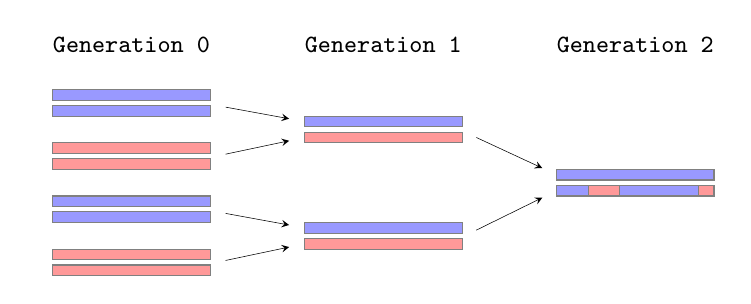
\begin{tikzpicture}[yscale=0.09, xscale=0.2]

\tikzset{
pop1/.style={fill=blue!40,draw=black!50},
pop2/.style={fill=red!40,draw=black!50},
inherit/.style={->,>=stealth,ultra thin,shorten <=2mm,shorten >=2mm,very thin},
recomb/.style={thick,draw=black!70}
}

% Nodes
\node (hapx) at (1,0) {};
\node (hapy) at (0,1.5) {};
\node (hapxy) at ($10*(hapx) + (hapy)$) {};

\node (gen1) at (0,0) {};
\node (gen2) at ($8*(hapx) + 0*(hapx)$) {};
\node (gen3) at ($8*(hapx) + 8*(hapx)$) {};

\node (ind1gen3) at ($(gen3) + (0,0)$) {};
\node (indsep) at ($5*(hapy)$) {};

\node (ind1gen2) at ($(gen2) + 1*(indsep)$) {};
\node (ind2gen2) at ($(gen2) - 1*(indsep)$) {};

\node (ind1gen1) at ($(gen1) + 1.5*(indsep)$) {};
\node (ind2gen1) at ($(gen1) + 0.5*(indsep)$) {};
\node (ind3gen1) at ($(gen1) - 0.5*(indsep)$) {};
\node (ind4gen1) at ($(gen1) - 1.5*(indsep)$) {};

\node (chr1) at ($0.25*(hapy)$)  {};
\node (chr2) at ($-1.25*(hapy)$) {};


% Haplotypes

\filldraw[pop1] ($(gen1) + (ind1gen1) + (chr1)$) rectangle +(hapxy);
\filldraw[pop1] ($(gen1) + (ind1gen1) + (chr2)$) rectangle +(hapxy);

\filldraw[pop2] ($(gen1) + (ind2gen1) + (chr1)$) rectangle +(hapxy);
\filldraw[pop2] ($(gen1) + (ind2gen1) + (chr2)$) rectangle +(hapxy);

\filldraw[pop1] ($(gen1) + (ind3gen1) + (chr1)$) rectangle +(hapxy);
\filldraw[pop1] ($(gen1) + (ind3gen1) + (chr2)$) rectangle +(hapxy);

\filldraw[pop2] ($(gen1) + (ind4gen1) + (chr1)$) rectangle +(hapxy);
\filldraw[pop2] ($(gen1) + (ind4gen1) + (chr2)$) rectangle +(hapxy);


\filldraw[pop1] ($(gen2) + (ind1gen2) + (chr1)$) rectangle +(hapxy);
\filldraw[pop2] ($(gen2) + (ind1gen2) + (chr2)$) rectangle +(hapxy);

\filldraw[pop1] ($(gen2) + (ind2gen2) + (chr1)$) rectangle +(hapxy);
\filldraw[pop2] ($(gen2) + (ind2gen2) + (chr2)$) rectangle +(hapxy);


\filldraw[pop1] ($(gen3) + (ind1gen3) + (chr1)$) rectangle +(hapxy);
\fill[pop1] ($(gen3) + (ind1gen3) + (chr2)$) rectangle +(hapxy);
\fill[pop2] ($(gen3) + (ind1gen3) + (chr2)+ 2*(hapx)$) rectangle ($(gen3) + (ind1gen3) + (chr2)+ (hapxy)$);
\fill[pop1] ($(gen3) + (ind1gen3) + (chr2)+ 4*(hapx)$) rectangle ($(gen3) + (ind1gen3) + (chr2)+ (hapxy)$);
\fill[pop2] ($(gen3) + (ind1gen3) + (chr2)+ 9*(hapx)$) rectangle ($(gen3) + (ind1gen3) + (chr2)+ (hapxy)$);
%\draw ($(gen3) + (ind1gen3) + (chr2)$) rectangle +(hapxy);


% Copying lines

\node (startline) at ($-1*(hapx) + 0.5*(hapy)$) {};
\node (chrdiff) at ($(chr1) - (chr2)$) {};


% Arrows
\draw[inherit] ($(gen1) + (ind1gen1) + (chr2) + 10*(hapx) + 0.75*(chrdiff)$) -- ($(gen2) + (ind1gen2) + (chr1) + 0.5*(hapy)$);
\draw[inherit] ($(gen1) + (ind2gen1) + (chr2) + 10*(hapx) + 0.75*(chrdiff)$) -- ($(gen2) + (ind1gen2) + (chr2) + 0.5*(hapy)$);
\draw[inherit] ($(gen1) + (ind3gen1) + (chr2) + 10*(hapx) + 0.75*(chrdiff)$) -- ($(gen2) + (ind2gen2) + (chr1) + 0.5*(hapy)$);
\draw[inherit] ($(gen1) + (ind4gen1) + (chr2) + 10*(hapx) + 0.75*(chrdiff)$) -- ($(gen2) + (ind2gen2) + (chr2) + 0.5*(hapy)$);

\draw[inherit] ($(gen2) + (ind1gen2) + (chr2) + 10*(hapx) + 0.75*(chrdiff)$) -- ($(gen3) + (ind1gen3) + (chr1) + 0.5*(hapy)$);
\draw[inherit] ($(gen2) + (ind2gen2) + (chr2) + 10*(hapx) + 0.75*(chrdiff)$) -- ($(gen3) + (ind1gen3) + (chr2) + 0.5*(hapy)$);


% Labels
\node (lab1) at ($(gen1) + 2.5*(indsep) + 0.5*(hapxy)$) {\small $\texttt{Generation 0}$};
\node (lab2) at ($2*(gen2) + 2.5*(indsep) + 0.5*(hapxy)$) {\small $\texttt{Generation 1}$};
\node (lab3) at ($4*(gen2) + 2.5*(indsep) + 0.5*(hapxy)$) {\small $\texttt{Generation 2}$};

%%%%%%%%%%%%%%%%%%%%%
% Identity-by-descent
% Nodes
\node (hapx) at (1,0) {};
\node (hapy) at (0,1.5) {};
\node (hapxy) at ($10*(hapx) + (hapy)$) {};

\node (gen1) at (0,0) {};
\node (gen2) at ($8*(hapx) + 0*(hapx)$) {};
\node (gen3) at ($8*(hapx) + 8*(hapx)$) {};

\node (ind1gen3) at ($(gen3) + (0,0)$) {};
\node (indsep) at ($5*(hapy)$) {};

\node (ind1gen2) at ($(gen2) + 1*(indsep)$) {};
\node (ind2gen2) at ($(gen2) - 1*(indsep)$) {};

\node (ind1gen1) at ($(gen1) + 1.5*(indsep)$) {};
\node (ind2gen1) at ($(gen1) + 0.5*(indsep)$) {};
\node (ind3gen1) at ($(gen1) - 0.5*(indsep)$) {};
\node (ind4gen1) at ($(gen1) - 1.5*(indsep)$) {};

\node (chr1) at ($0.25*(hapy)$)  {};
\node (chr2) at ($-1.25*(hapy)$) {};


\end{tikzpicture}
}
 \end{subcolumns}
 \end{columns}

%%% BLOCK 1
     \begin{columns}%blocks will be placed into columns
         \column{.5}
         \block[roundedcorners=40,titleoffsety=-8cm,bodyoffsety=-8cm,bodyverticalshift=-1cm]{1. Tree sequences}{
Genetic sequence data is BIG and REPETITIVE:\\[2mm]

\begin{center}
{\tt
%\ldots GTAACGCGATAAGA\Cvermillion{G}ATTAGCCCAAAAACACAGACATGG\Cvermillion{A}AATAGCGTA\ldots \\
%\ldots GTAACGCGATAAGA\Cvermillion{G}ATTAGCCCAAAAACACAGACATGG\Cvermillion{A}AATAGCGTA\ldots \\
\ldots GTAACGCGATAAGA\Cvermillion{G}ATTAGCCCAAAAACACAGACATGG\Cvermillion{A}AATAGCGTA\ldots \\
\ldots GTAACGCGATAAGA\Cvermillion{G}ATTAGCCCAAAAACACAGACATGG\Cvermillion{A}AATAGCGTA\ldots \\
\ldots GTAACGCGATAAGA\Cskyblue{T}ATTAGCCCAAAAACACAGACATGG\Cvermillion{A}AATAGCGTA\ldots \\
\ldots GTAACGCGATAAGA\Cskyblue{T}ATTAGCCCAAAAACACAGACATGG\Cvermillion{A}AATAGCGTA\ldots \\
\ldots GTAACGCGATAAGA\Cskyblue{T}ATTAGCCCAAAAACACAGACATGG\Cvermillion{A}AATAGCGTA\ldots \\
\ldots GTAACGCGATAAGA\Cskyblue{T}ATTAGCCCAAAAACACAGACATGG\Cskyblue{T}AATAGCGTA\ldots \\
%\ldots GTAACGCGATAAGA\Cskyblue{T}ATTAGCCCAAAAACACAGACATGG\Cskyblue{T}AATAGCGTA\ldots \\
%\ldots GTAACGCGATAAGA\Cskyblue{T}ATTAGCCCAAAAACACAGACATGG\Cskyblue{T}AATAGCGTA\ldots \\
\ldots GTAACGCGATAAGA\Cskyblue{T}ATTAGCCCAAAAACACAGACATGG\Cskyblue{T}AATAGCGTA\ldots \\[1mm]
}
\gray{\small $\leftarrow 5\times 10^7$ bases for small human chromosome $\rightarrow$}\\[4mm]
\end{center}
%Because of this, you are probably used to storing your data in a compressed format, and decompressing it only when you need to perform analyses or query the data. Doing this can be time-consuming and computationally expensive, however.
%Storing $n = 1\times 10^5$ chromosomes in a compressed VCF requires $\approx$ 50 GB.
However, common haplotypes in a sample are often simply a consequence of some common history. So if we know this history (as we always do in simulations!), storing it directly is often more convenient and efficient than storing the raw haplotypes. This is the key idea behind the \magenta{tree sequence} data structure [1], which encodes a complete genealogy for a sample of chromosomes at each chromosomal location. Tree sequences offer a few benefits to population geneticists compared with traditional sequence-based file formats:

\begin{itemize}
\item They can store large simulated datasets extremely compactly.

\item As they hold rich detail about the history of the sample, many important processes can be observed directly from the tree structure.

\item They can be queried and modified extremely quickly.
\end{itemize}
     }
     
     %%%% BLOCK 3
     \block[titleoffsety=1cm,bodyoffsety=4cm]{3. Example: total IBD sharing over time}{
     } 
\centering
  \begin{subcolumns}
  \subcolumn{.48}
  \block{}{
  \centering
  

%% Set up the document
%\documentclass[convert={density=300,size=1080x800,outext=.png}]{standalone}
%
%% Include any extra LaTeX packages required
%%\usepackage[square, numbers, comma, sort&compress]{natbib}  % Use the "Natbib" style for the references in the Bibliography
%
%\usepackage{verbatim}  % Needed for the "comment" environment to make LaTeX comments
%\usepackage[table,x11names]{xcolor} % needed for highlighted rows
%
%\usepackage{tabularx,booktabs,adjustbox} % For tables
%\usepackage{pdflscape} % For writing some pages in landscape mode
%\usepackage{afterpage} % For control over the positioning of figures and tables.
%
%% For pictures
%\usepackage{tikz}
%\usetikzlibrary{calc,fit,arrows,decorations.pathmorphing,backgrounds,fit,positioning}
%\usetikzlibrary{shapes.symbols}
%
%% tikz colour settings
%\tikzset{pop0/.style={red!50!yellow},pop1/.style={violet!80},pop2/.style={olive!70!green}}
%
%%% ----------------------------------------------------------------
%\begin{document}
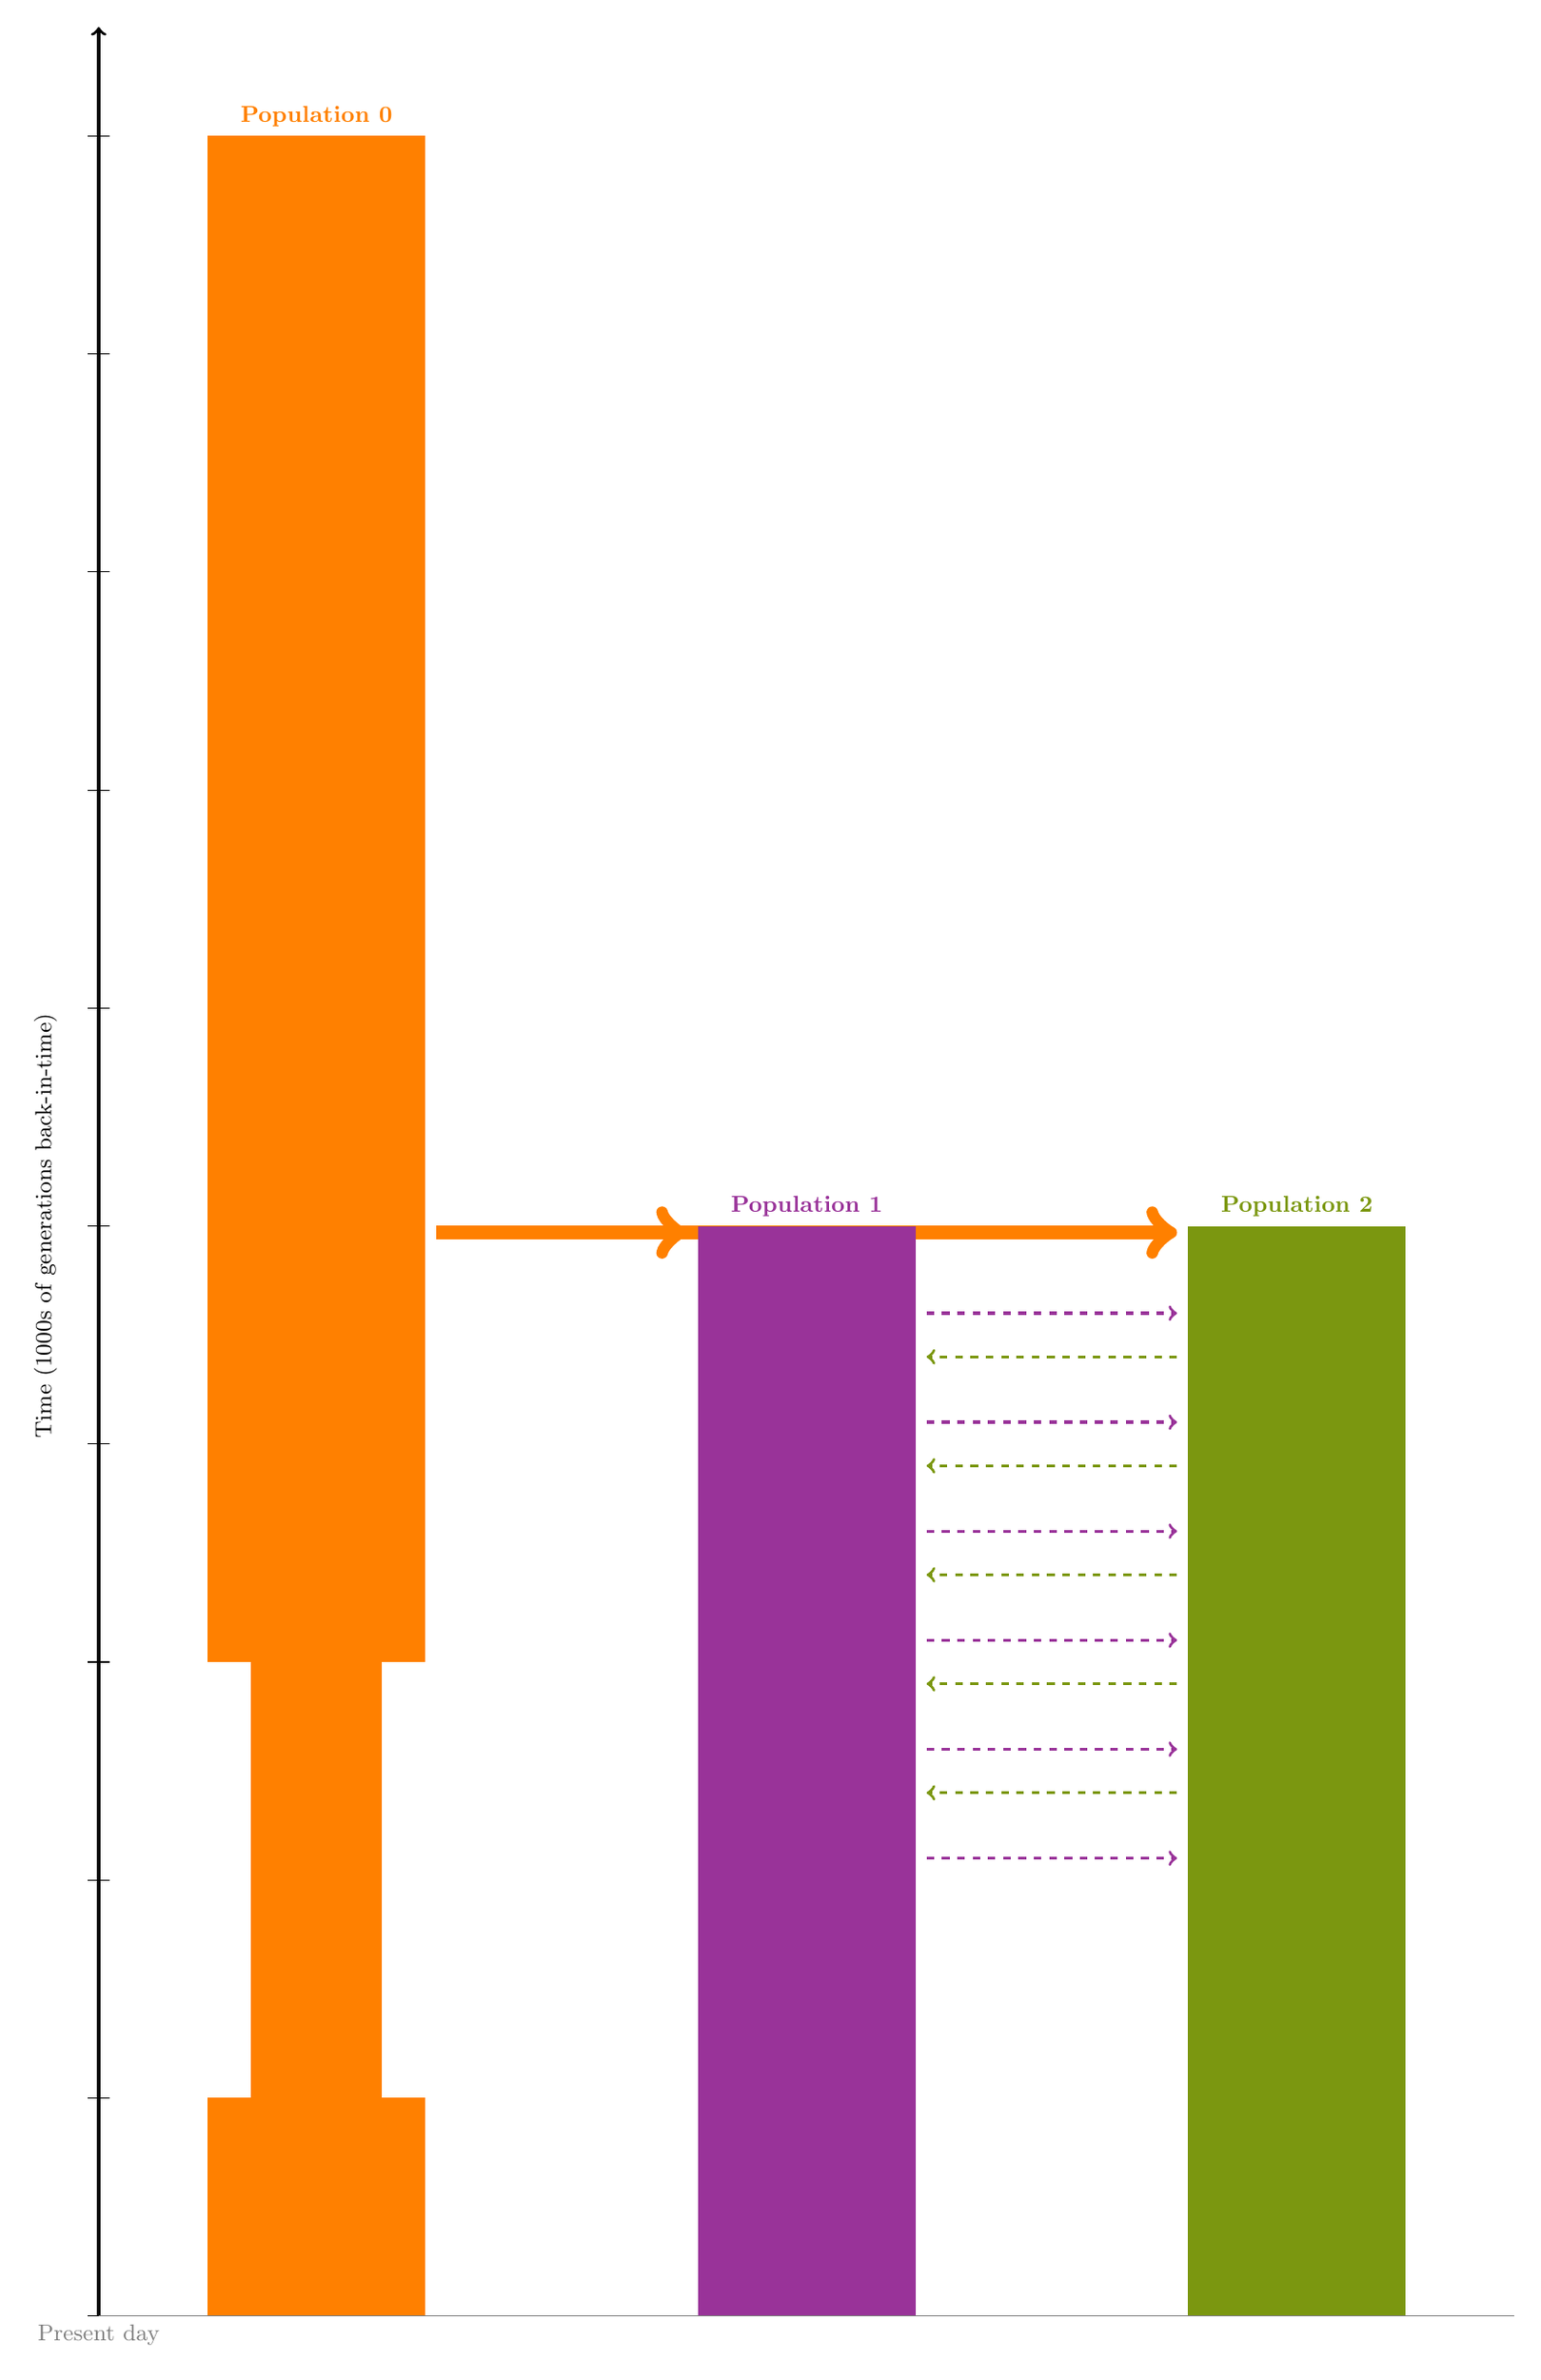
\begin{tikzpicture}[node distance=5mm and 5mm, xscale=1.5, yscale=3]

\tikzset{greynode/.style={font=\footnotesize,node distance=1cm and 1 cm,fill=black!10,draw=black!30,inner sep=0pt,minimum size=3.5mm,shape=circle},
mutations/.style={shape=starburst,fill=red!50!blue,inner sep=0.8pt,starburst points=11,starburst point height=.2cm}}

% Nodes
\node (origin) at (0,0){};
\node (pop0) at (1,0){};
\node (pop1) at (5.5,0){};
\node (pop2) at (10,0){};
\node (popwidth) at (2,0){};

% Axis
\node (leftAx) at (-1,0) {};
\draw[very thick,->] (-1,0) -- +(0, 10.5);
\foreach \y in {0, 1, 2, 3, 4, 5, 6, 7, 8, 9, 10} \draw ($(leftAx) + (-0.1, \y)$) -- ($(leftAx) + (0.1, \y)$); % tick marks
%\node[anchor=east] at ($(leftAx)$) {0}; \node[anchor=east] at ($(leftAx) + (0,5)$) {5};
\node[rotate=90,anchor=south] (leftLabel) at ($(leftAx) + (-0.3,5)$) {\small$\textrm{Time (1000s of generations back-in-time)}$};

% Migrations
\foreach \y in {1.5,2,2.5,3,3.5,4} \draw[pop1,dashed,->,very thick] ($(.1,.1) + (leftAx) + (0,\y + .5)+(pop1) + (popwidth)$) -- +(2.3,0);
\foreach \y in {2,2.5,3,3.5,4} \draw[pop2,dashed,->,very thick] ($(-.1,-.1) + (leftAx) + (0,\y + .5)+(pop2)$) -- +(-2.3,0);
\draw[pop0, ->, line width=2mm] ($(.1,0) + (leftAx) + (0,4.97)+(pop0) + (popwidth)$) -- +(2.3,0);
\draw[pop0, ->, line width=2mm] ($(.1,0) + (leftAx) + (0,4.97)+(pop0) + 2*(popwidth)$) -- +($2*(2.4,0)$);

% Populations
\foreach \x in {0} \fill[pop\x] ($(leftAx) + (pop\x)$) -- ++(0,10) -- ++(2, 0) -- ++(0, -10) -- cycle;
\foreach \x in {1, 2} \fill[pop\x] ($(leftAx) + (pop\x)$) -- ++(0,5) -- ++(2, 0) -- ++(0, -5) -- cycle;
\foreach \x in {0} \node[above,pop\x] (label\x) at ($(leftAx) + (pop\x) + (1, 10)$) {\small\bf Population \x};
\foreach \x in {1,2} \node[above,pop\x] (label\x) at ($(leftAx) + (pop\x) + (1, 5)$) {\small\bf Population \x};

% Times
\draw[very thin,color=gray] (-1,0) node[below] {\small Present day} -- (12,0);

% White squares over pop0 bottleneck areas.
\fill[white] ($(leftAx) + 0.9*(pop0) + (0,1)$) -- ++($0.5*(pop0)$) -- ++(0,2) -- ++($-0.5*(pop0)$) -- cycle;
\fill[white] ($(leftAx) + 1.1*(pop0) +(popwidth) + (0,1)$) -- ++($-0.5*(pop0)$) -- ++(0,2) -- ++($0.5*(pop0)$) -- cycle;

% Grey dashed arrows
%\foreach \y in {2,4,6,8,10} \draw[gray,densely dashed,->] ($(12,\y)$) -- +(4,0);

\end{tikzpicture} 
%\end{document}  % The End
%%% ----------------------------------------------------------------
%  \input{pics/new-method/simulation-method-0.tex}
%    \input{pics/new-method/simulation-method-2.tex}
%      \input{pics/new-method/simulation-method-4.tex}
  }
  \subcolumn{.35}
   \block{}{
   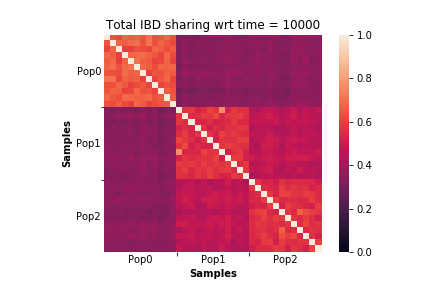
\includegraphics[scale=.63]{pics/kinships-10000.png}
   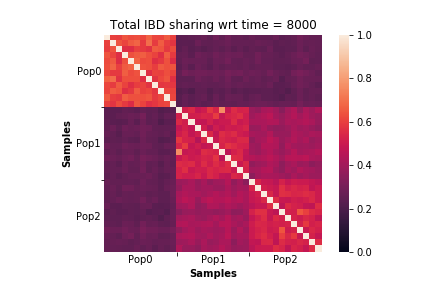
\includegraphics[scale=.63]{pics/kinships-8000.png}
    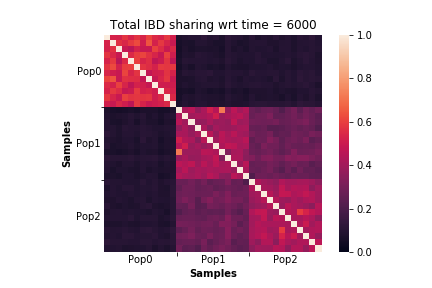
\includegraphics[scale=.63]{pics/kinships-6000.png}
    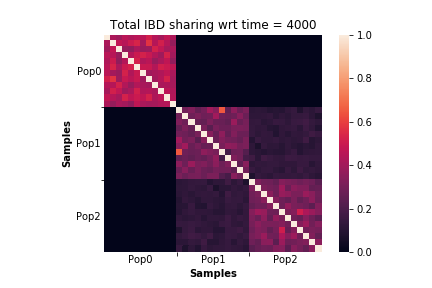
\includegraphics[scale=.63]{pics/kinships-4000.png}
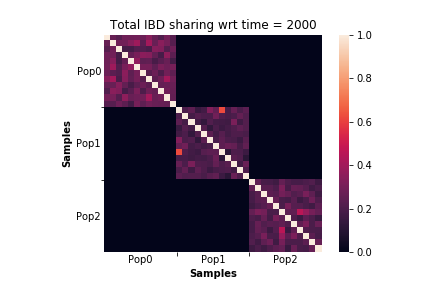
\includegraphics[scale=.63]{pics/kinships-2000.png}

  }
  \end{subcolumns}



     \column{.5}
     %%% BLOCK 2
         \block[titleoffsety=-8cm,bodyoffsety=-3.5cm]{2. IBD and ancestry in tree sequences}{}  
%          \begin{subcolumns}       
%         \subcolumn{.45}
          \block{}{
          \begin{center}
          \begin{center}
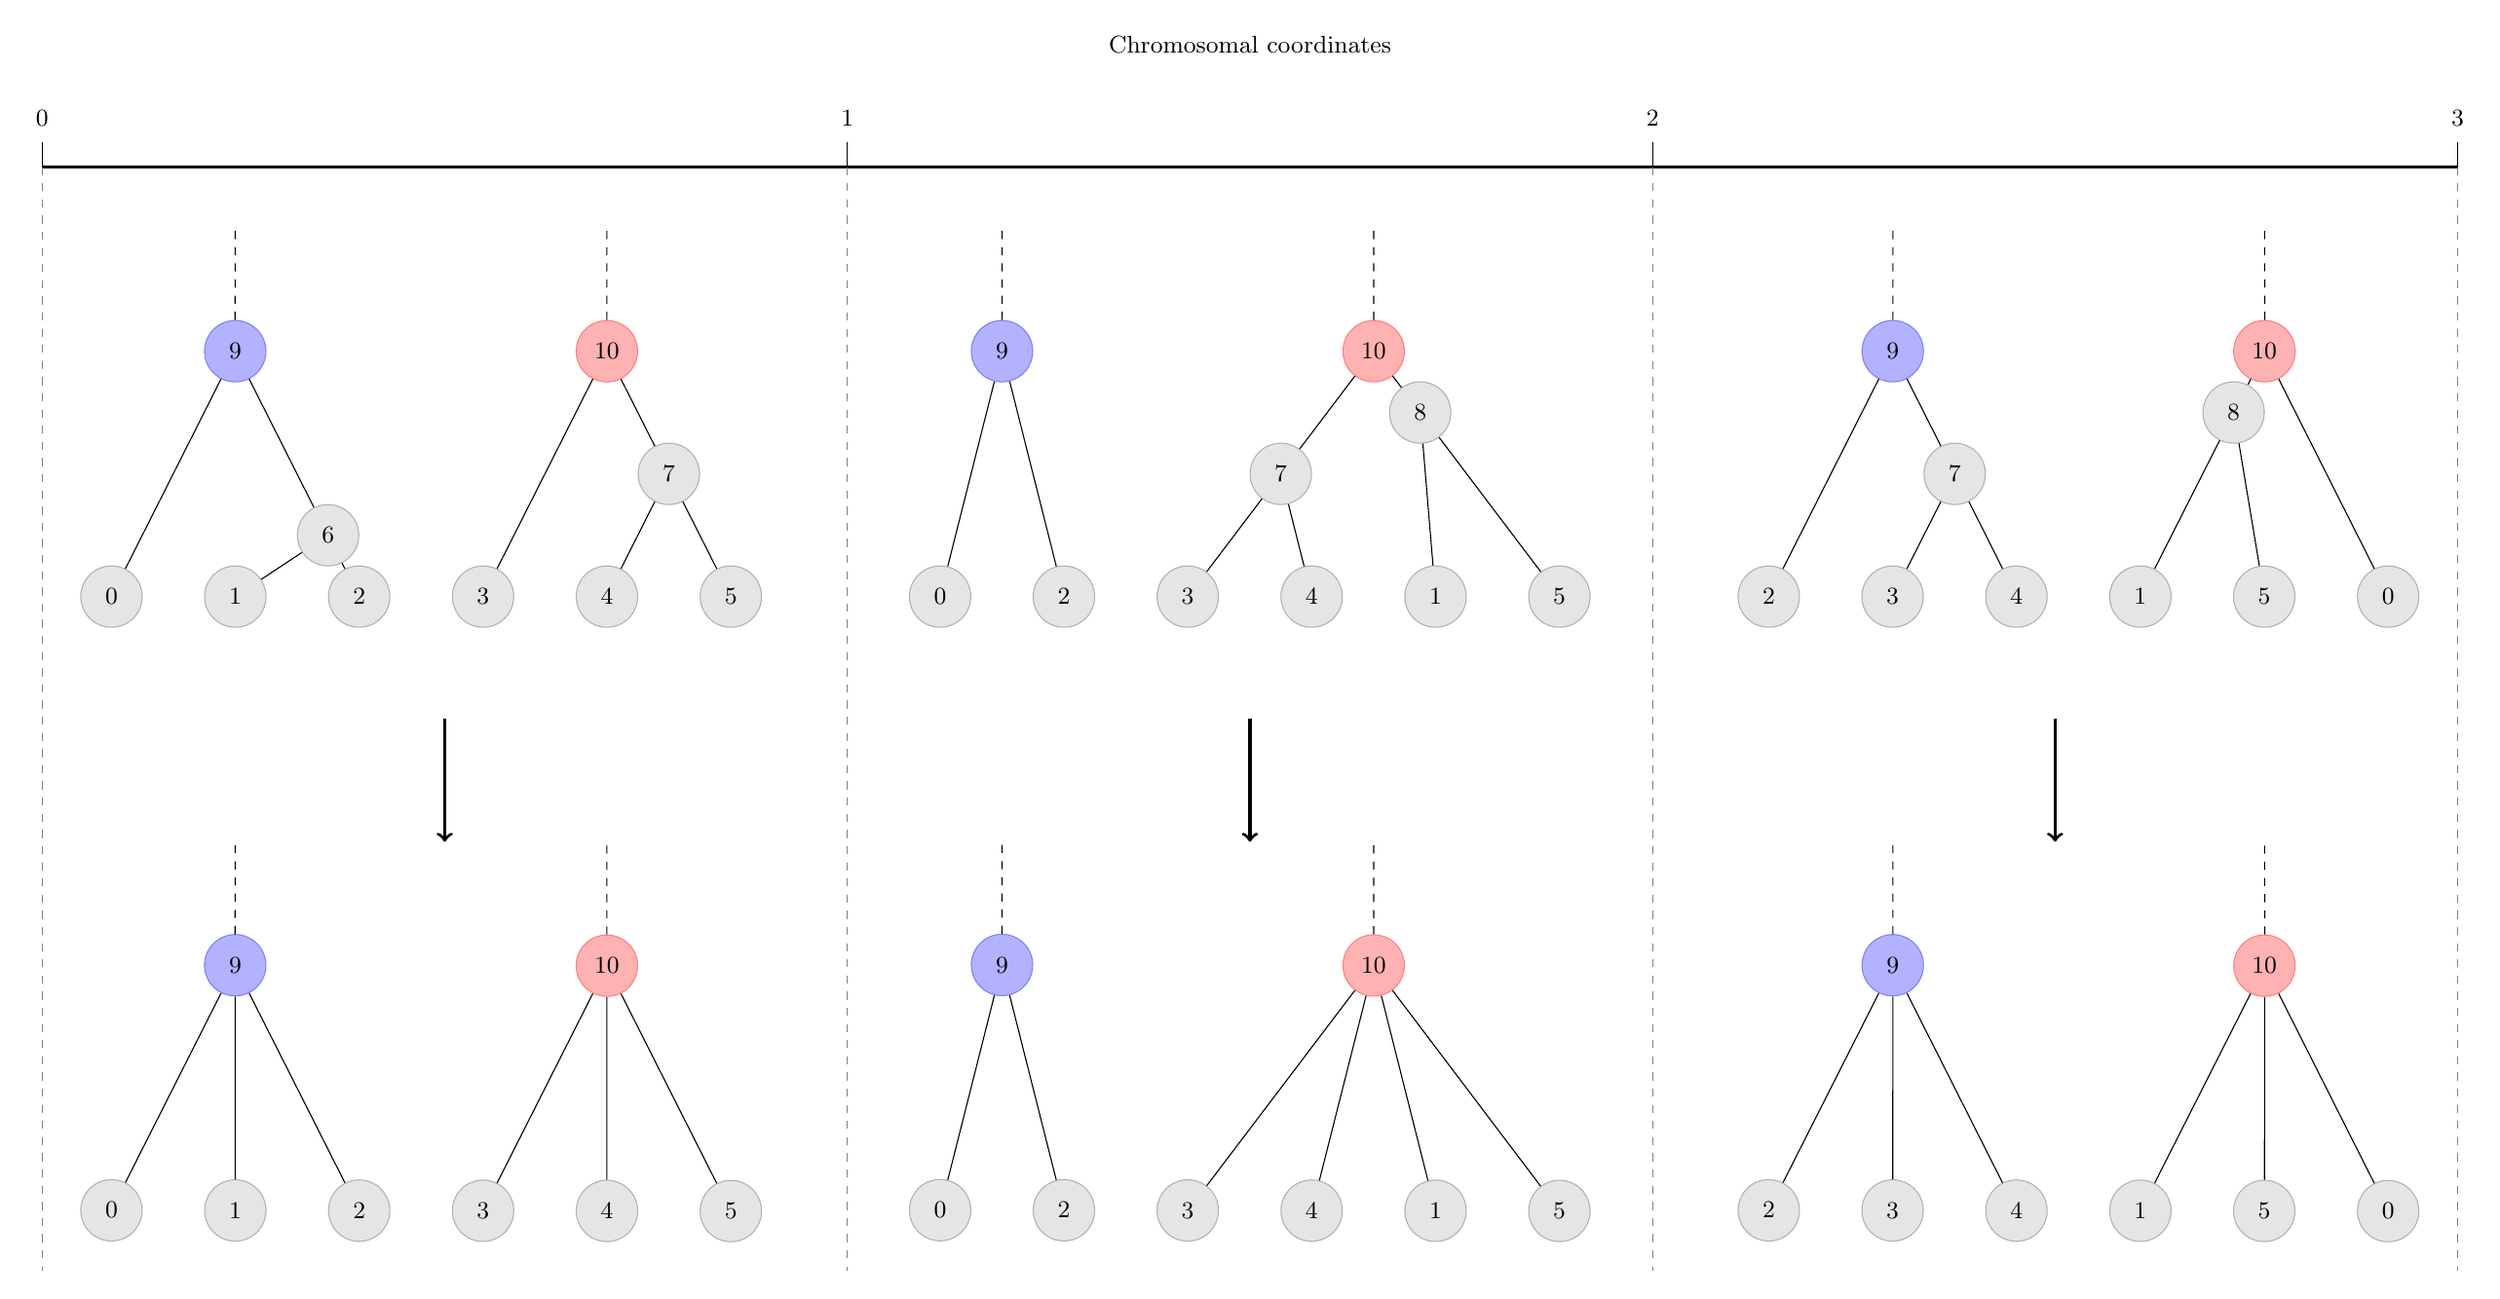
\begin{tikzpicture}[node distance=8mm and 8mm,xscale=1.8,yscale=1.6]

\tikzset{greynode/.style={font=\small,node distance=.5cm and .5 cm,fill=black!10,draw=black!30,inner sep=0pt,minimum size=8mm,shape=circle},
bluenode/.style={font=\small,node distance=.5cm and .5cm,fill=blue!30,draw=blue!50,inner sep=0pt,minimum size=8mm,shape=circle},
rednode/.style={font=\small,node distance=.5cm and .5cm,fill=red!30,draw=red!50,inner sep=0pt,minimum size=8mm,shape=circle}}

% Middle sample nodes
\node (s0) [greynode] {0};
\node (s2) [right=of s0,greynode] {2};
\node (s3) [right=of s2,greynode] {3};
\node (s4) [right=of s3,greynode] {4};
\node (s1) [right=of s4,greynode] {1};
\node (s5) [right=of s1,greynode] {5};

% Left sample nodes
\node (leftTree) at (-6, 0) {};
\node[greynode] (s0l) at ($(s0) + (leftTree)$) {0};
\node[greynode] (s1l) at ($(s2) + (leftTree)$) {1};
\node[greynode] (s2l) at ($(s3) + (leftTree)$) {2};
\node[greynode] (s3l) at ($(s4) + (leftTree)$) {3};
\node[greynode] (s4l) at ($(s1) + (leftTree)$) {4};
\node[greynode] (s5l) at ($(s5) + (leftTree)$) {5};

% Right sample nodes
\node (rightTree) at (6, 0) {};
\node [greynode] (s2r) at ($(s0) + (rightTree)$) {2};
\node [greynode] (s3r) at ($(s2) + (rightTree)$) {3};
\node [greynode] (s4r) at ($(s3) + (rightTree)$) {4};
\node [greynode] (s1r) at ($(s4) + (rightTree)$) {1};
\node [greynode] (s5r) at ($(s1) + (rightTree)$) {5};
\node [greynode] (s0r) at ($(s5) + (rightTree)$) {0};

% Ancestral nodes
\node (anc) at (0,2) {};
\node[bluenode] (s9) at ($0.5*(s0) + 0.5*(s2) + (anc)$) {9};
\node[bluenode] (s9l) at ($0.5*(s0l) + 0.5*(s2l) + (anc)$) {9};
\node[bluenode] (s9r) at ($0.5*(s2r) + 0.5*(s4r) + (anc)$) {9};
\node[rednode] (s10) at ($0.5*(s3)+0.5*(s5) + (anc)$) {10};
\node[rednode] (s10l) at ($0.5*(s3l)+0.5*(s5l) + (anc)$) {10};
\node[rednode] (s10r) at ($0.5*(s1r)+0.5*(s0r) + (anc)$) {10};

% Internal nodes
\node[greynode] (s6l) at ($(s2l)!0.25!(s9l)$) {6};
\node[greynode] (s7) at ($(s3)!.5!(s10)$) {7};
\node[greynode] (s7l) at ($(s5l)!.5!(s10l)$) {7};
\node[greynode] (s7r) at ($(s4r)!.5!(s9r)$) {7};
\node[greynode] (s8) at ($(s5)!.75!(s10)$) {8};
\node[greynode] (s8r) at ($(s1r)!.75!(s10r)$) {8};

% Edges
\draw (s0) -- (s9) -- (s2); \draw (s3) -- (s7) -- (s10) -- (s8) -- (s5); \draw (s4) -- (s7); \draw (s1) -- (s8); % middle tree
\draw (s0l) -- (s9l) -- (s6l) -- (s2l); \draw (s1l) -- (s6l); \draw ( s3l) -- (s10l) -- (s7l) -- (s5l); \draw (s4l) -- (s7l); % left tree
\draw (s2r) -- (s9r) -- (s7r) -- (s4r); \draw (s3r) -- (s7r); \draw (s1r) -- (s8r) -- (s10r) -- (s0r); \draw (s5r) -- (s8r); % right tree
\draw[dashed] (s9) -- +(0,1); \draw[dashed] (s9l) -- +(0,1); \draw[dashed] (s9r) -- +(0,1);
\draw[dashed] (s10) -- +(0,1); \draw[dashed] (s10l) -- +(0,1); \draw[dashed] (s10r) -- +(0,1);

% Axes
\node (topAx) at (0,3.5) {};
\node (topLeft) at ($(s0l) + (topAx) + (-0.5, 0)$) {};
\node (topRight) at ($(s0r) + (topAx) + (0.5,0)$) {};
\draw[very thick] (topLeft.center) -- (topRight.center);
\node (genunit) at ($0.3333*(topRight) - 0.3333*(topLeft)$) {};
\foreach \x in {0,1,2,3} \draw ($(topLeft) + \x*(genunit)$) -- +(0,.2);
\foreach \x in {0,1,2,3} \node at ($(topLeft) + \x*(genunit) + (0,.4)$) {\small\x};

% Interval endpoints
\foreach \x in {0,1,2,3} \draw[thin,color=black!50,dashed] ($(topLeft) + \x*(genunit)$) -- +(0, -9);
%\draw[thin,color=black!50,dashed] ($(topLeft) + 7*(genUnit)$) -- +(0, -5.5);

% Axis titles
\node (topLabel) at ($(topLeft) + 1.5*(genunit) + (0,1)$) {\small$\textrm{Chromosomal coordinates}$};

%%%%%
\node (after) at (0, -5) {};

% Middle sample nodes
\node[greynode] (s0) at (after) {0};
\node (s2) [right=of s0,greynode] {2};
\node (s3) [right=of s2,greynode] {3};
\node (s4) [right=of s3,greynode] {4};
\node (s1) [right=of s4,greynode] {1};
\node (s5) [right=of s1,greynode] {5};

% Left sample nodes
\node (leftTree) at (-6, 0) {};
\node[greynode] (s0l) at ($(s0) + (leftTree)$) {0};
\node[greynode] (s1l) at ($(s2) + (leftTree)$) {1};
\node[greynode] (s2l) at ($(s3) + (leftTree)$) {2};
\node[greynode] (s3l) at ($(s4) + (leftTree)$) {3};
\node[greynode] (s4l) at ($(s1) + (leftTree)$) {4};
\node[greynode] (s5l) at ($(s5) + (leftTree)$) {5};

% Right sample nodes
\node (rightTree) at (6, 0) {};
\node [greynode] (s2r) at ($(s0) + (rightTree)$) {2};
\node [greynode] (s3r) at ($(s2) + (rightTree)$) {3};
\node [greynode] (s4r) at ($(s3) + (rightTree)$) {4};
\node [greynode] (s1r) at ($(s4) + (rightTree)$) {1};
\node [greynode] (s5r) at ($(s1) + (rightTree)$) {5};
\node [greynode] (s0r) at ($(s5) + (rightTree)$) {0};

% Ancestral nodes
\node (anc) at (0,2) {};
\node[bluenode] (s9) at ($0.5*(s0) + 0.5*(s2) + (anc)$) {9};
\node[bluenode] (s9l) at ($0.5*(s0l) + 0.5*(s2l) + (anc)$) {9};
\node[bluenode] (s9r) at ($0.5*(s2r) + 0.5*(s4r) + (anc)$) {9};
\node[rednode] (s10) at ($0.5*(s3)+0.5*(s5) + (anc)$) {10};
\node[rednode] (s10l) at ($0.5*(s3l)+0.5*(s5l) + (anc)$) {10};
\node[rednode] (s10r) at ($0.5*(s1r)+0.5*(s0r) + (anc)$) {10};

%% Axes
%\node (topAx) at (0,3.5) {};
%\node (topLeft) at ($(s0l) + (topAx) + (-0.5, 0)$) {};
%\node (topRight) at ($(s0r) + (topAx) + (0.5,0)$) {};
%\draw[very thick] (topLeft.center) -- (topRight.center);
%\node (genunit) at ($0.3333*(topRight) - 0.3333*(topLeft)$) {};
%\foreach \x in {0,1,2,3} \draw ($(topLeft) + \x*(genunit)$) -- +(0,.2);
%\foreach \x in {0,1,2,3} \node at ($(topLeft) + \x*(genunit) + (0,.4)$) {\x};

% Edges
\draw (s0) -- (s9) -- (s2); \draw (s3) -- (s10) -- (s4); \draw (s1) -- (s10) --  (s5); % middle tree
\draw (s0l) -- (s9l) -- (s2l); \draw (s1l) -- (s9l); \draw (s3l) -- (s10l) -- (s5l); \draw (s4l) -- (s10l); % left tree
\draw (s2r) -- (s9r) -- (s3r); \draw (s4r) -- (s9r); \draw (s1r) -- (s10r) -- (s5r); \draw (s0r) -- (s10r);

\draw[dashed] (s9) -- +(0,1); \draw[dashed] (s9l) -- +(0,1); \draw[dashed] (s9r) -- +(0,1);
\draw[dashed] (s10) -- +(0,1); \draw[dashed] (s10l) -- +(0,1); \draw[dashed] (s10r) -- +(0,1);

% Interval endpoints
\foreach \x in {0,1,2,3} \draw[thin,color=black!50,dashed] ($(topLeft) + \x*(genunit)$) -- +(0, -4);
%\draw[thin,color=black!50,dashed] ($(topLeft) + 7*(genUnit)$) -- +(0, -5.5);

%% Axis titles
%\node (topLabel) at ($(topLeft) + 1.5*(genunit) + (0,1)$) {$\textrm{Chromosomal coordinates}$};

%% Arrows
\foreach \x in {0, 1, 2} \draw[<-,very thick] ($(topLeft) + \x*(genunit) + 0.5*(genunit) + (0,-5.5)$) -- +(0, 1);

\end{tikzpicture}
\end{center} 
          \end{center}
          By assigning population labels to the nodes that correspond to ancestors of the sample, tree sequences can store the sample's local ancestry. 
          The branch joining a sample node to an ancestral node shows its ancestry.
          Extracting this information efficiently is challenging due to correlations in genealogical structure between samples, and across chromosomes; 
          in an upcoming paper, we will describe an algorithm that enables us to do this.
          }           
       
\vspace{20cm}

             \block[titleoffsety=-2.5cm,bodyoffsety=-2.5cm]{4. Method performance}{
             \begin{center}
%\large
\centering
\setlength{\aboverulesep}{5pt}
\setlength{\belowrulesep}{5pt}
%\newcolumntype{R}{>{\raggedleft\arraybackslash}X}%
\begin{tabularx}{.45\textwidth}{p{8cm}p{7cm}p{7cm}p{7cm}X}
\toprule
%& \multicolumn{3}{c}{{\bf Global ancestry}} \\[1mm]
 & Missing data & Run time (sec) &  File size (Mb) & Selection \\
\midrule 
{\bf \texttt{msprime}} & $4.0$\% & 6 & 9 & No \\ \addlinespace
{\bf \texttt{msprime}} +~ARG & $0.0$\% & 53  & 1700  & No\\ \addlinespace
%{\bf + migration records} & $0.0$\% &  & & \crossmark \\ 
%\midrule
%{\bf \texttt{SLiM}} & $4.0$\% & 10 min & 16 Mb  & \checkmark \\ \addlinespace
{\bf \texttt{SLiM}}& {$0.0$\%} & $>3600$  &  41 & {Yes} \\ \addlinespace
%\midrule
{\bf\magenta{\texttt{slime}}} & \magenta{$0.0$\%} & \magenta{86} & \magenta{39}  & \magenta{Yes} \\ \addlinespace
\bottomrule\\
\end{tabularx}
\end{center}
To illustrate the power of our method, \texttt{slime} [3], we simulated a toy demographic scenario inspired by the history of Neanderthal introgression into the Eurasian population.
We simulated 200 chromosomes of length $50\thinspace$Mb from 100 present-day Eurasian individuals, assuming a 2\% introgression of Neanderthals into Eurasians 2500 generations ago.
For simplicity, we assumed a constant effective population sizes of 5000 individuals, a uniform recombination rate of $1 \times  10^{-8}$ bp per generation, a uniform mutation rate of $1 \times  10^{-8}$  bp per generation and neutral variation.  
However, note that all of these methods can deal with more complexity than this.
In particular, both \texttt{slime} and \texttt{SLiM} are capable of simulating under selection.\\

Although still under development, \texttt{slime} appears to outperform existing tree sequence simulation softwares on various metrics by orders of magnitude.
As a principled fusion of \texttt{SLiM} and \texttt{msprime}, \texttt{slime} will allow users to track local ancestry in large simulations under realistically complex demographic scenarios, and with minimal computational overhead.
}

     \end{columns}

%%% BLOCK 5
 \block[titleoffsety=-3cm,bodyoffsety=-3cm]{5. Acknowledgements, references and further information}{
 }
  \begin{columns}
 \begin{subcolumns}
    \subcolumn{25} \block[bodyoffsetx=1.5cm,bodyverticalshift=-5cm]{}{
     GT is funded by the Helen Freeman scholarship, the Maurice Belz Fund and the Australian Government's Research Training Scheme. \\[1mm]
     [1] Kelleher, J., et al. (2016). Efficient Coalescent Simulation and Genealogical Analysis for Large Sample Sizes. PLOS Computational Biology, 12(5).\\[1mm]
     [2] Galloway, J.,  et al. (2018). Tree-sequence recording in SLiM opens new horizons for forward-time simulation of whole genomes. Molecular Ecology Resources, (November 2018), 552–566.\\[1mm]    
     [3] Under development: \texttt{https://github.com/gtsambos/slime}
     }
       \subcolumn{3} \block[bodyoffsetx=-3cm,bodyverticalshift=-8cm]{}{
       \begin{center}
       
\includegraphics[scale=1.2]{pics/unimelb-logo.jpg}
      \end{center}
       }
        \subcolumn{3} \block[bodyoffsetx=-5cm,bodyverticalshift=-7cm]{}{
       \begin{center}
       
\includegraphics[scale=1]{pics/GT_headshot.jpg}\\   
       Come say hi!
       \end{center}
       }
 \end{subcolumns}
 \end{columns}         

 \end{document}




\endinput
%%
%% End of file `tikzposter-example.tex'.
